\section{Udvælgelse af gestik-par til at justere lydstyrken}
\label{TestresultaterVolumen}
%
Udvælgelsen af hvilket gestik-par, der skal knyttes til at justere lydstyrken foretages på baggrund af testpersonernes begrundelser for til- og fravalg af de foreslåede gestikker. Der fokuseres først på, hvilke gestik-par testpersonerne har inddraget i deres top tre rangering og i den forbindelse, om det er muligt at ekskludere nogle gestik-par. Derefter fokuseres der på testpersonernes begrundelser for, hvorfor de har valgt de gestik-par, som de har, hvorunder forbedringsforslag inkluderes, hvis testpersonerne fremsætter nogle. Afsnittet vil afslutningsvist ende ud i hvilket gestik-par, der vælges til at justere lydstyrken.\blankline
%
Få at få et overblik over, hvor ofte de ni forskellige gestik-par individuelt indgår på enten en første-, anden- eller tredjeplads i top tre rangeringen opstilles følgende \autoref{fig:SamletTopTreVolumen}.
%
\begin{figure}[H]
	\centering
	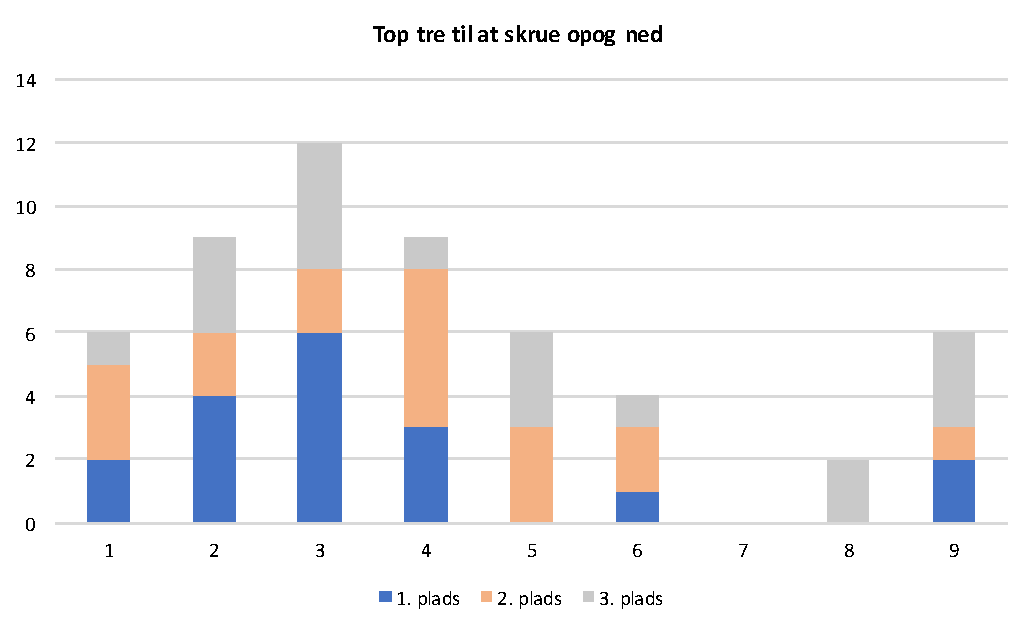
\includegraphics[resolution=300,width=0.9\textwidth]{Test1/DatabehandlingGrafer/TopTreVolumen}
	\caption{Søjlediagram over hvordan hvert gestik-par indgår i testpersonernes top tre i forhold til at justere lydstyrken. Data forefindes i \autoref{app:TopTreRangeringVolumen}.}
	\label{fig:SamletTopTreVolumen}
\end{figure}
\noindent
%
På \autoref{fig:SamletTopTreVolumen} fremgår det tydeligt, at GP2, GP3 samt GP4 er de tre gestik-par, som uafhængigt af den specifikke plads, indgår flest gange i testpersonernes top tre. Efterfulgt af GP1, GP5 og GP9. Derudover tyder det på, at hverken GP6, GP7 eller GP8 er specielt eftertragtet, da de henholdvis kun indgår fire, aldrig og to gange i testpersonernes samlede top tre, jævnfør \autoref{fig:SamletTopTreVolumen}. For at vurdere om der er belæg for, at ekskludere et eller flere gestik-par opstilles følgende \autoref{fig:DaarligstGestikVolumen}. 
%
\begin{figure}[H]
	\centering
	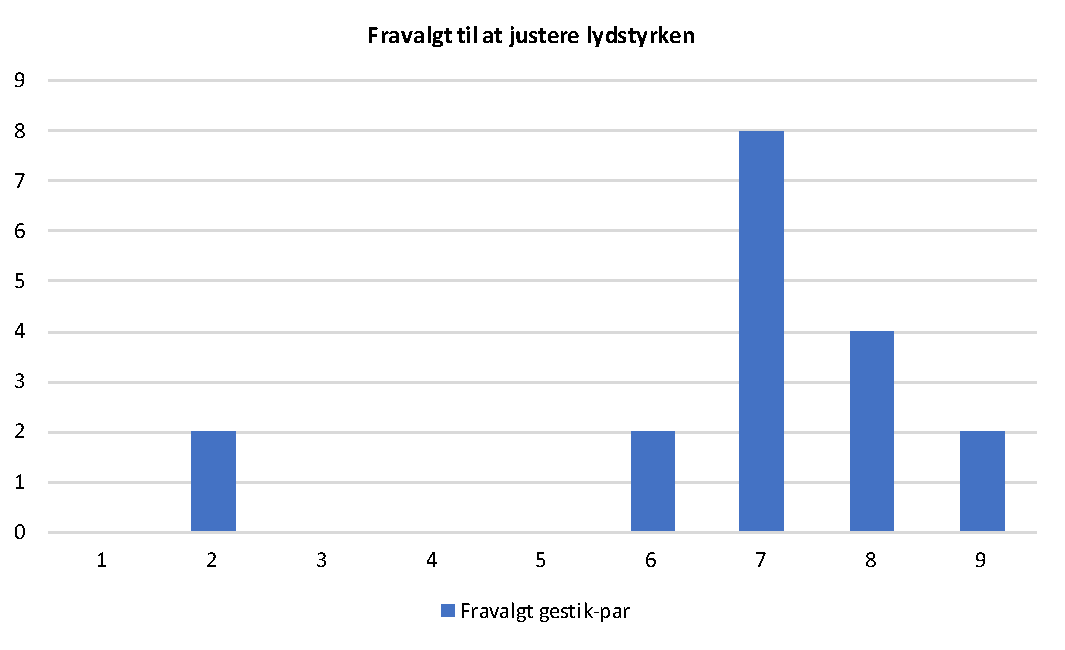
\includegraphics[resolution=300,width=0.9\textwidth]{Test1/DatabehandlingGrafer/FravalgtVolumen}
	\caption{Søjlediagram over hvilke gestik-par testpersonerne fravælger i forbindelse med at justere lydstyrken.}
	\label{fig:DaarligstGestikVolumen}
\end{figure}
\noindent
%
På \autoref{fig:DaarligstGestikVolumen} opsummeres antallet af gange hvert gestik-par fravælges af testpersonerne. Da otte ud af 18 testpersoner har fravalgt GP7 konkluderes det, at testpersonerne ikke bryder sig om GP7, hvorfor GP7 ekskluderes. På \autoref{fig:SamletTopTreVolumen} fremgår det, at GP8 hverken tildeles en første- eller andenplads og derudover kun indgår to gange på en tredjeplads og da GP8 fravælges af fire testpersoner, vurderes det, at GP8 er overflødig og irrelevant. Der er derfor belæg for at ekskludere GP8. Tilsvarende er gældende for GP6, som kun indgår fire gange i testpersonernes samlede top tre og kun tildeles en førsteplads én gang, jævnfør \autoref{fig:SamletTopTreVolumen}, og derudover fravælges to gange, jævnfør \autoref{fig:DaarligstGestikVolumen}. Der er derfor belæg for at ekskludere GP6. I \autoref{app:TestresultaterVolumenDaarlig} forefindes en dybere analyse af hvorfor testpersonerne fravælger de gestik-par, som de gør. 

Ekskluderingen af de tre gestik-par medfører, at den efterfølgende analyse vil omhandle testpersonernes begrundelser for at vælge GP1, GP2, GP3, GP4, GP5 samt GP9.
%
\subsection{Testpersonernes begrundelse for valg af gestik-par 1}
\label{TestresultaterValgAfGestikkerBegrundelseGP1Volumen}
%
Med udgangspunkt i \autoref{fig:SamletTopTreVolumen} tildeles GP1 en førsteplads af to testpersoner, en andenplads af tre testpersoner og en tredjeplads af én testperson. GP1 illustreres på \autoref{fig:GestikPar1Volumen}. De testpersoner, som har tildelt GP1 en førsteplads, begrunder det med, at det er en velkendt bevægelse; at dreje på en knap for at skrue op. Derudover påpeger TP8 både, at bevægelsen i GP1 er tydeligere sammenlignet med GP2 og at GP1 er naturlig. I tillæg påpeger TP16, at bevægelsen i GP1 så mere behagelig ud sammenlignet med GP2, som testpersonen fandt ukomfortabel. 

En af årsagerne til at TP16 vurderer, at GP2 er ukomfortabel, skyldes formentlig, at GP2 i videooptagelsen ikke gengives lige så afslappet, som det er hensigten. I videooptagelsen fremgår det, at hele armen skal i bevægelse; fra skulderen ud til fingrene, hvilket ikke er hensigten med GP2. Hensigten med GP2 er derimod, at bevægelsen dannes ud fra en kombination mellem underarm, håndled og fingre, så det tilnærmelsesvist er den samme bevægelse som ved GP1. Sammenholdes TP16's udsagn med testpersonens bevægelser, når testpersonen opfordres til at fremsætte et forbedringsforslag, så gengiver TP16 GP2 og det er først når testlederen konfronterer TP16, at testpersonen gengiver GP1. Afslutningsvist gengiver TP16 ikke GP1, men noget der tilnærmelsesvist minder om GP2 bortset fra, at fingrene er udstrakt og roteres i en cirkulær bevægelse. Da hverken testpersonens udsagn eller bevægelser stemmer overens med GP1, indikerer det, at TP16 formentligt foretrækker noget, der i højere grad minder om GP2, men særligt foretrækkes en cirkulær bevægelse.
%
\begin{figure}[H]
	\centering
	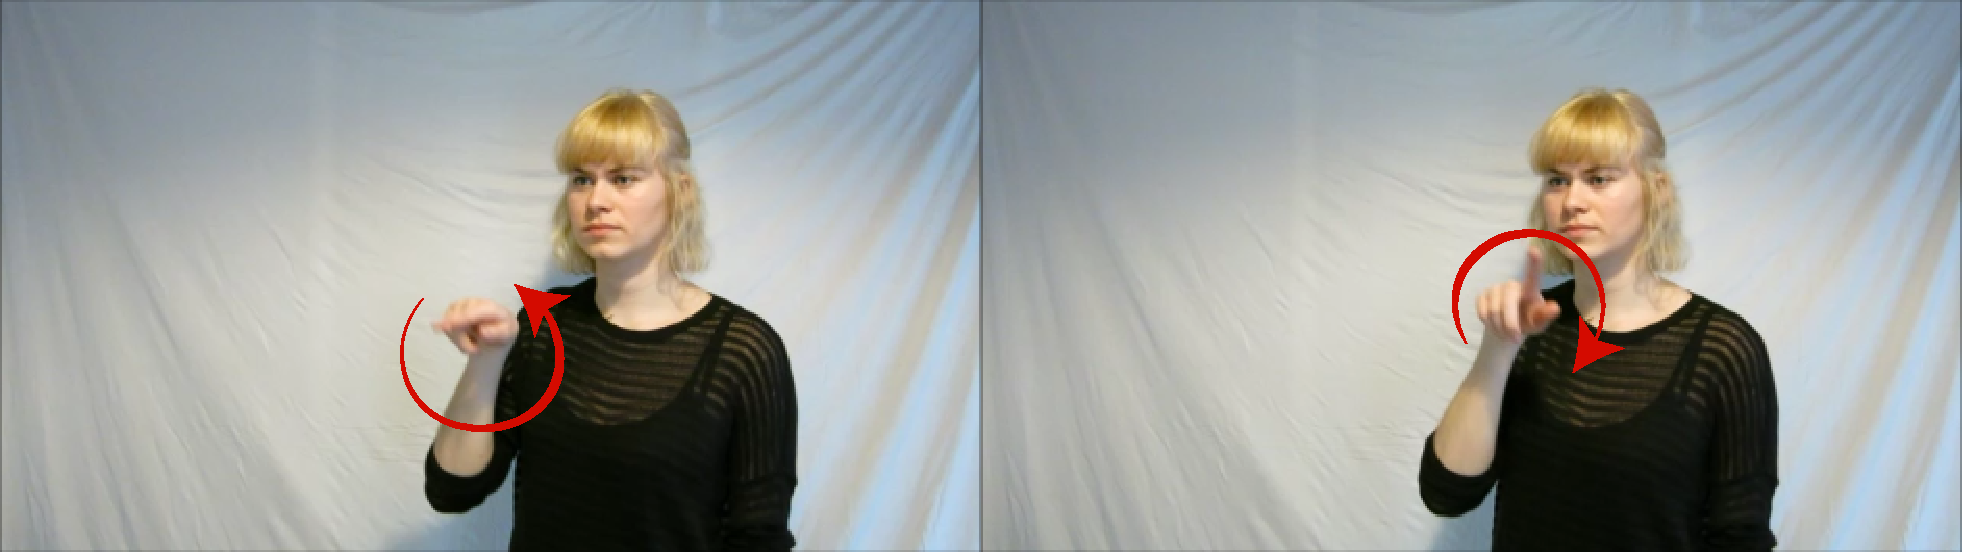
\includegraphics[resolution=300,width=0.9\textwidth]{Test1/Gestik-par/Gestik1_Volumen}
	\caption{Illustration af gestik-par 1; cirkulær bevægelse med pegefingeren i urets retning for at skrue op og mod uret for at skrue ned.}
	\label{fig:GestikPar1Volumen}
\end{figure}
\noindent
%
Da der kun er to testpersoner, som har tildelt GP1 en førsteplads og det er begrænset hvilke egenskaber de foretrækker ved GP1, vurderes det, at det er nødvendigt at inddrage de resterende fire testpersoner, som har inkluderet GP1 i deres top tre. De testpersoner, som har tildelt GP1 en anden- eller tredjeplads, begrunder det ud fra en kombination af følgende egenskaber: 
%
\begin{multicols}{3}
    \begin{itemize}
        \item Naturlig bevægelse
        \item Intuitiv 
        \item Nem at forstå
        \item Universel
        \item Nem
        \item Overskuelig
        \item Cirkulær bevægelse
        \item Kræver én hånd
\end{itemize}
\end{multicols}
\noindent
%
Derudover kommenterer TP4, at både GP1 og GP2 er gestikker, der kan forbindes direkte til at justere lydstyrken. Ifølge TP5 kan bevægelsen i GP1 gengives overalt samt i forskellige størrelser. Selvom TP5 ikke inkluderer GP2 i sin top tre, så giver TP5 udtryk for godt at kunne lide, hvad testpersonen definerer som volumenknappen, svarende til GP2. Årsagen til at GP2 ikke indgår i TP5's top tre skyldes, ifølge testpersonen, at GP2 er langsom at gengive sammenlignet med GP1. Fælles for både TP9 og TP13 er, at de begge foretrækker gestikker, hvor det kun kræver én hånd at gengive dem. Derudover kommenterer TP13 at cirkulære bevægelser er sjove og at de minder om en knap, hvilket ligeledes er gældende for GP2.      
%
\subsection{Testpersonernes begrundelse for valg af gestik-par 2}
\label{TestresultaterValgAfGestikkerBegrundelseGP2Volumen}
%
Med udgangspunkt i \autoref{fig:SamletTopTreVolumen} tildeles GP2 en førsteplads af fire testpersoner, en andenplads af to testpersoner og en tredjeplads af tre testpersoner. GP2 illustreres på \autoref{fig:GestikPar2Volumen}. De fire testpersoner, som har tildelt GP2 en førsteplads, begrunder det ud fra en kombination af følgende egenskaber: 
%
\begin{multicols}{3}
    \begin{itemize}
        \item Naturlig bevægelse
        \item Giver mening
        \item Intuitiv 
        \item Nem at huske
        \item Behageligt at dreje
        \item Cirkulær bevægelse
        \item Kræver én hånd
        \item Specifik
\end{itemize}
\end{multicols}
\noindent
%
Ifølge TP1, så tænkte testpersonen på GP2 før testpersonen blev præsenteret for gestik-parret. Som tidligere nævnt, vælger TP14 gestikker ud fra, hvad der ikke naturligt forekommer, når testpersonen normaltvist gestikulerer, hvorfor TP14 tildeler GP2 førstepladsen. Lignende argumenter fremsættes af TP18, som påpeger, at fordi bevægelsen i GP2 er så specifik, så er det ikke en bevægelse, der fejlagtigt gengives. 
%
\begin{figure}[H]
	\centering
	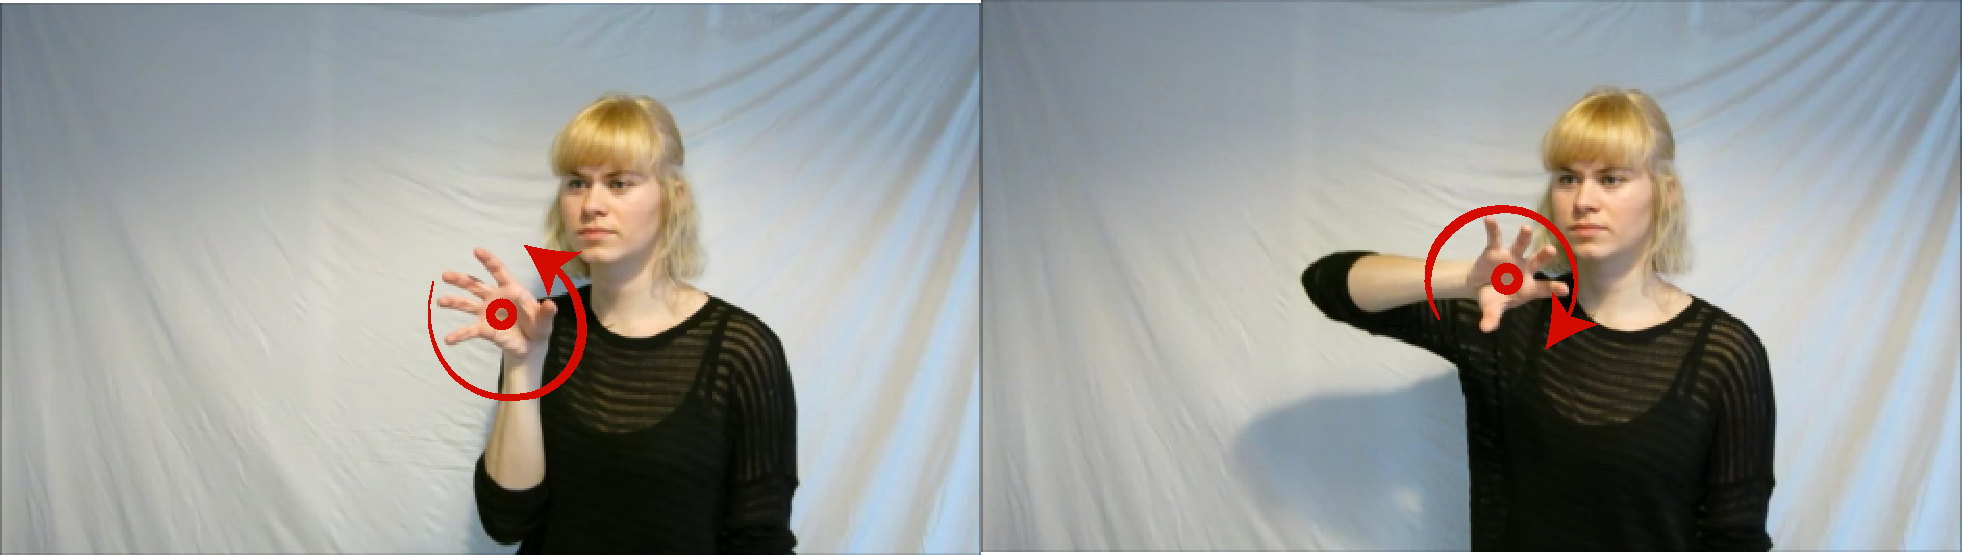
\includegraphics[resolution=300,width=0.9\textwidth]{Test1/Gestik-par/Gestik2_Volumen}
	\caption{Illustration af gestik-par 2; cirkulær bevægelse med halv bøjede fingrene, ligesom hvis det er en drejeknap, der blev brugt. Der skal drejes med uret for at skrue op og mod uret for at skrue ned.}
	\label{fig:GestikPar2Volumen}
\end{figure}
\noindent
%
Den generelle tendens er, at GP2 forbindes med en drejeknap, hvor seks ud af ni testpersoner, som har inkluderet GP2 i deres top tre, decideret giver udtryk for den forbindelse. Tendensen udledes, blandt andet, af følgende to citater: 
%
\begin{quotation}
	\noindent
	\textit{2'eren, fordi det synes jeg virker mest naturligt, det er ligesom at dreje på en knap, som man gør på gamle stereoanlæg.} TP1, \autoref{app:NoterValgAfGestikker}.
\noindent
\end{quotation}
% 
%
\begin{quotation}
	\noindent
	\textit{Jeg synes også 2'eren giver mening sådan i forhold til at skrue op for en volumen-knap.} TP3, \autoref{app:NoterValgAfGestikker}.
\noindent
\end{quotation}
%
En af fordelene ved at vælge GP2 fremfor GP1 er, at GP2 oftere indgår i testpersonernes samlede top tre, jævnfør \autoref{fig:SamletTopTreVolumen}. Det anses ydermere for at være en fordel, at flere testpersoner forbinder GP2 med en drejeknap, som normalvist benyttes til at justere lydstyrken på et musikanlæg eller en forstærker. Det er en fordel, fordi testpersonerne dermed kan overføre den fysiske, velkendte interaktion med en drejeknap til en interaktion baseret på gestikker. Ud fra testpersonernes erfaring med drejeknapper, behøver de ikke at lære noget nyt. Endvidere påpeger både TP14 og TP18 at bevægelsen i GP2 ikke er en bevægelse, der normalvist indgår i ens naturlige kropssprog. 
%
\subsubsection{Forbedringsforslag til gestik-par 2}
\label{TestresultaterValgAfGestikkerForbedringGP2Volumen}
%
Udover at bevægelsesmængden i GP2 ikke behøver at være så udtryksfuld, som det illustreres i videooptagelsen, er der kun to testpersoner, som fremsætter et forbedringsforslag. TP14 foreslår, at den ikke-dominante hånd; hånden, som ikke foretager cirkelbevægelsen, inkluderes, hvilket resulterer i, at det kræver begge hænder at justere lydstyrken. Da størstedelen af testpersonerne foretrækker gestikker, som kun kræver én hånd, afvises foreslaget, men det tages til eftertrakning, at der måske skal være et nyt element i GP2. Et forslag til det nye element fremsættes af TP1, som foreslår, at hånden først er lukket sammen i en knytnæve og når hånden åbnes, kan lydstyrken justeres via GP2. Det nye element i GP2 skal ikke nødvendigvis være den knyttede næve, men kan derimod være en anden form for indikation af, at brugeren tager fat i en fiktiv drejeknap. 

Fordelen ved at implementere en form for indikation, inden lydstyrken kan justeres, er, at det for teknologien kan blive nemmere at registrere, hvor meget lydstyrken justeres.\blankline
%    
Med forbehold for, at GP2 ikke nødvendigvis skal gengives i overensstemmelse med, hvordan GP2 gengives i videooptagelsen og at brugeren muligvis først skal indikere, at der efterfølgende vil være en justering af lydstyrken, så vurderes det, at GP2 egner sig bedre end GP1 til at justere lydstyrken. Derudover indgår GP2 oftere i testpersonernes samlede top tre i forhold til GP1, jævnfør \autoref{fig:SamletTopTreVolumen}. Med dette i betragtning vurderes det derfor, at der er belæg for at ekskludere GP1. 
%
\subsection{Testpersonernes begrundelse for valg af gestik-par 3}
\label{TestresultaterValgAfGestikkerBegrundelseGP3Volumen}
%
Med udgangspunkt i \autoref{fig:SamletTopTreVolumen} tildeles GP3 en førsteplads af seks testpersoner, en andenplads af to testpersoner og en tredjeplads af fire testpersoner. GP3 illustreres på \autoref{fig:GestikPar3Volumen}. De seks testpersoner, som har tildelt GP3 en førsteplads, begrunder det ud fra en kombination af følgende egenskaber: 
%
\begin{multicols}{3}
    \begin{itemize}
        \item Intuitiv
        \item Nem at huske
        \item Giver mening
        \item Logisk
        \item Simpel
        \item Naturlig
        \item Nem at udføre
        \item Kræver én hånd
\end{itemize}
\end{multicols}
\noindent
%
Derudover giver TP11 udtryk for, at hvis der skal skrues op for lydstyrken, bør det være med en opadgående bevægelse. Lignende argumenter forefindes ved TP13. Ifølge TP6 er det nemmere at gengive GP3 og GP4 sammenligt med GP5, som kræver begge hænder. TP4 tildelte GP3 førstpladsen ud fra, hvad der passede til testpersonens valg af gestik-par til pause og start; GP1. Da GP1 til pause og start blev ekskluderet, er det uvist, hvorvidt TP4 stadig vil tildele GP3 en førsteplads. 
%
\begin{figure}[H]
	\centering
	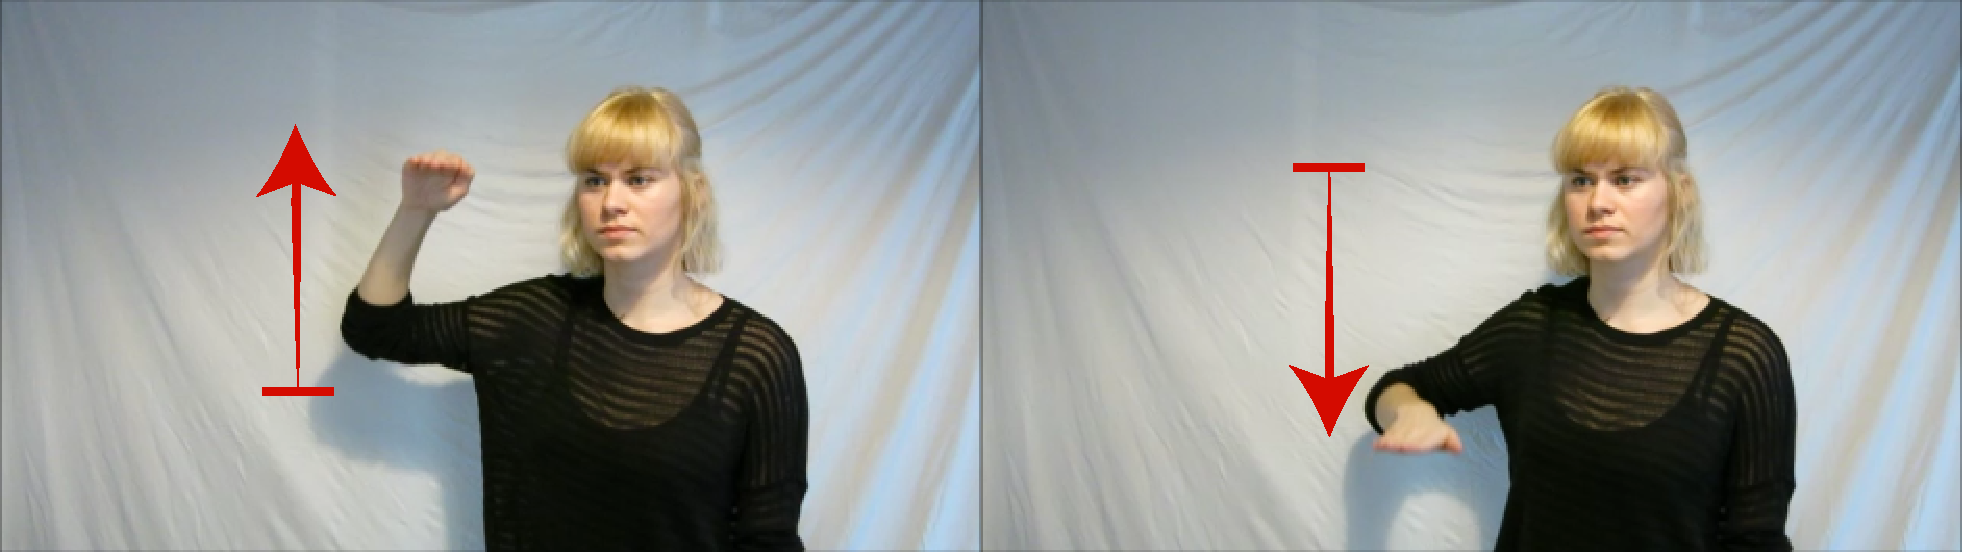
\includegraphics[resolution=300,width=0.9\textwidth]{Test1/Gestik-par/Gestik3_Volumen}
	\caption{Illustration af gestik-par 3; horisontal hånd løftes vertikalt med håndfladen nedad for at skrue op og for at skrue ned sænkes hånden vertikalt med håndfladen nedad.}
	\label{fig:GestikPar3Volumen}
\end{figure}
\noindent
%
Rettes fokus mod de testpersoner, som har tildelt GP3 en anden- eller tredjeplads, så begrundes det, foruden de listede egenskaber, med hvordan lyd visualiseres på en computer. TP17's begrundelse for, at tildele GP3 en tredjeplads er, at GP3 er en kombination af GP5 og GP9 i forhold til mængden af kontrol testpersonen har over justeringen af lydstyrken. \blankline
%      
Ud af de seks testpersoner, som har tildelt GP3 en førsteplads, er der ingen af dem, som begår fejl når de gengiver bevægelsen. Udover at GP3 gerne må udføres mere afslappet end hvad der gengives på \autoref{fig:GestikPar3Volumen}, så fremsætter ingen testpersoner forbedringsforslag.\blankline
%
Med udgangspunkt i testpersonernes udsagn og at GP3 indgår 12 gange i testpersonernes samlede top tre rangering, jævnfør \autoref{fig:SamletTopTreVolumen}, så forefindes der på nuværende tidspunkt ikke belæg for, at ekskludere GP3. 
%
\subsection{Testpersonernes begrundelse for valg af gestik-par 4}
\label{TestresultaterValgAfGestikkerBegrundelseGP4Volumen}
%
Med udgangspunkt i \autoref{fig:SamletTopTreVolumen} tildeles GP4 en førsteplads af tre testpersoner, en andenplads af fem testpersoner og en tredjeplads af én testperson. GP4 illustreres på \autoref{fig:GestikPar4Volumen}. De tre testpersoner, som har tildelt GP4 en førsteplads, begrunder det ud fra en kombination af følgende egenskaber: 
%
\begin{multicols}{3}
    \begin{itemize}
        \item Giver mening
        \item Tydelig indikation
        \item Simpel
        \item Kræver én hånd
\end{itemize}
\end{multicols}
\noindent
%
Derudover argumenterer TP18 for, at årsagen til at GP4 tildeles en førsteplads skyldes, at armen kun skal hæves eller sænkes og dermed ikke skal positioneres på en bestemt måde.
%
\begin{figure}[H]
	\centering
	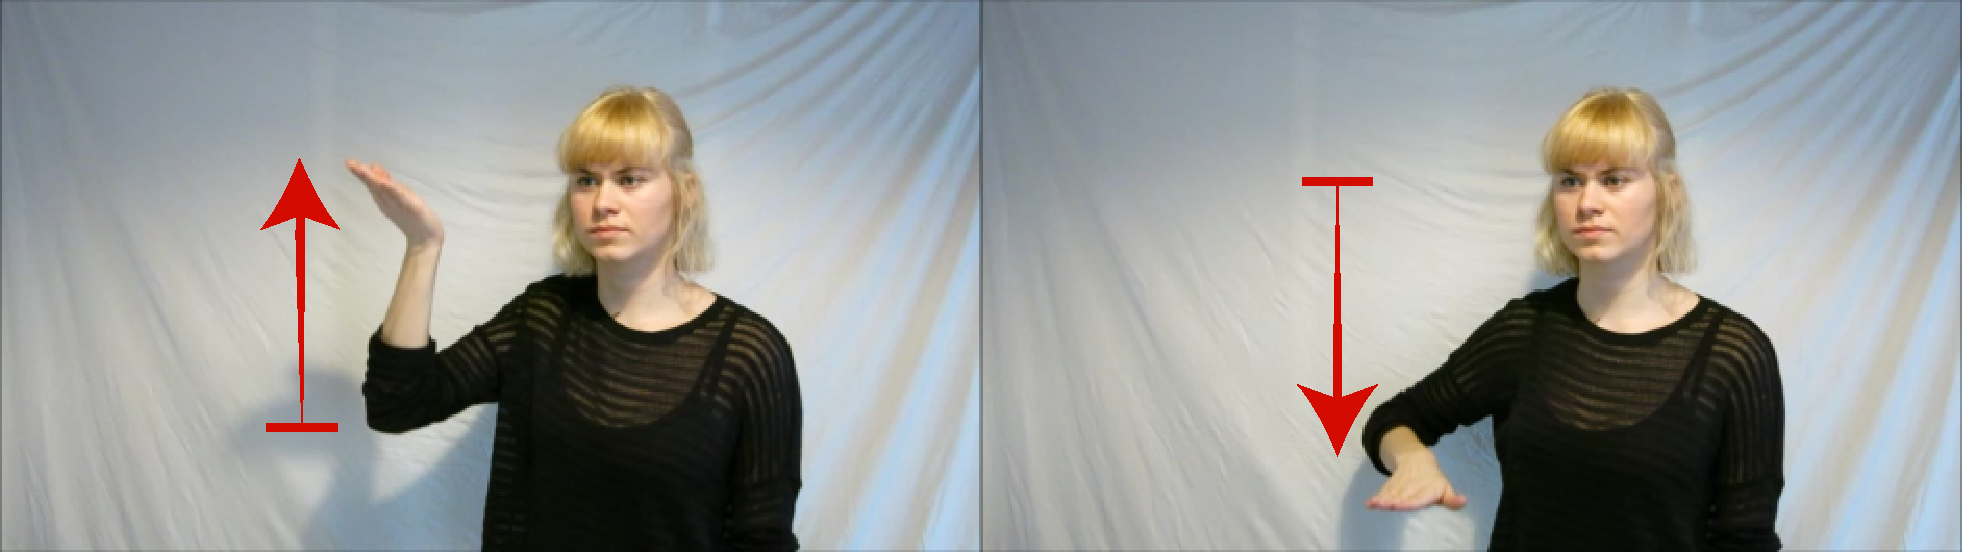
\includegraphics[resolution=300,width=0.9\textwidth]{Test1/Gestik-par/Gestik4_Volumen}
	\caption{Illustration af gestik-par 4; horisontal hånd løftes vertikalt med håndfladen opad for at skrue op og for at skrue ned sænkes hånden vertikalt med håndfladen nedad.}
	\label{fig:GestikPar4Volumen}
\end{figure}
\noindent
%
Fire ud af fem testpersoner, som har tildelt GP4 en andenplads, kommenterer, at GP4 minder om GP3. Dog pointerer TP11 og TP15 henholdvis, at der ikke bør skelnes mellem GP3 og GP4 og at GP4 er mere kompliceret end GP3. Derudover begrunder de fem testpersoner, som har tildelt GP4 en andenplads ud fra en kombination af følgende egenskaber: 
%
\begin{multicols}{3}
    \begin{itemize}
        \item Giver mening
        \item Intuitiv
        \item Logisk
        \item Simpel
\end{itemize}
\end{multicols}
\noindent
%
I tillæg kommenterer TP3, at det giver mening at løfte et eller andet op, i det her tilfælde lydstyrken, og derefter skubbe det ned igen, hvorfor en vertikal bevægelse er at foretrække over en horisontal bevægelse. Derudover lægger TP9, som har tildelt GP4 en tredjeplads, vægt på, hvad der er mindst krævende og mindst distraherende.\blankline 
%
Med udgangspunkt i på testpersonernes udsagn og at GP4 indgår ni gange i testpersonernes samlede top tre rangering, jævnfør \autoref{fig:SamletTopTreVolumen}, så forefindes der på nuværende tidspunkt ikke belæg for, at ekskludere GP4.
%
\subsection{Testpersonernes begrundelse for valg af gestik-par 5}
\label{TestresultaterValgAfGestikkerBegrundelseGP5Volumen}
% 
På \autoref{fig:SamletTopTreVolumen} fremgår det, at GP5 ikke tildeles en førsteplads én eneste gang. GP5 illustreres på \autoref{fig:GestikPar5Volumen}.  
%
\begin{figure}[H]
	\centering
	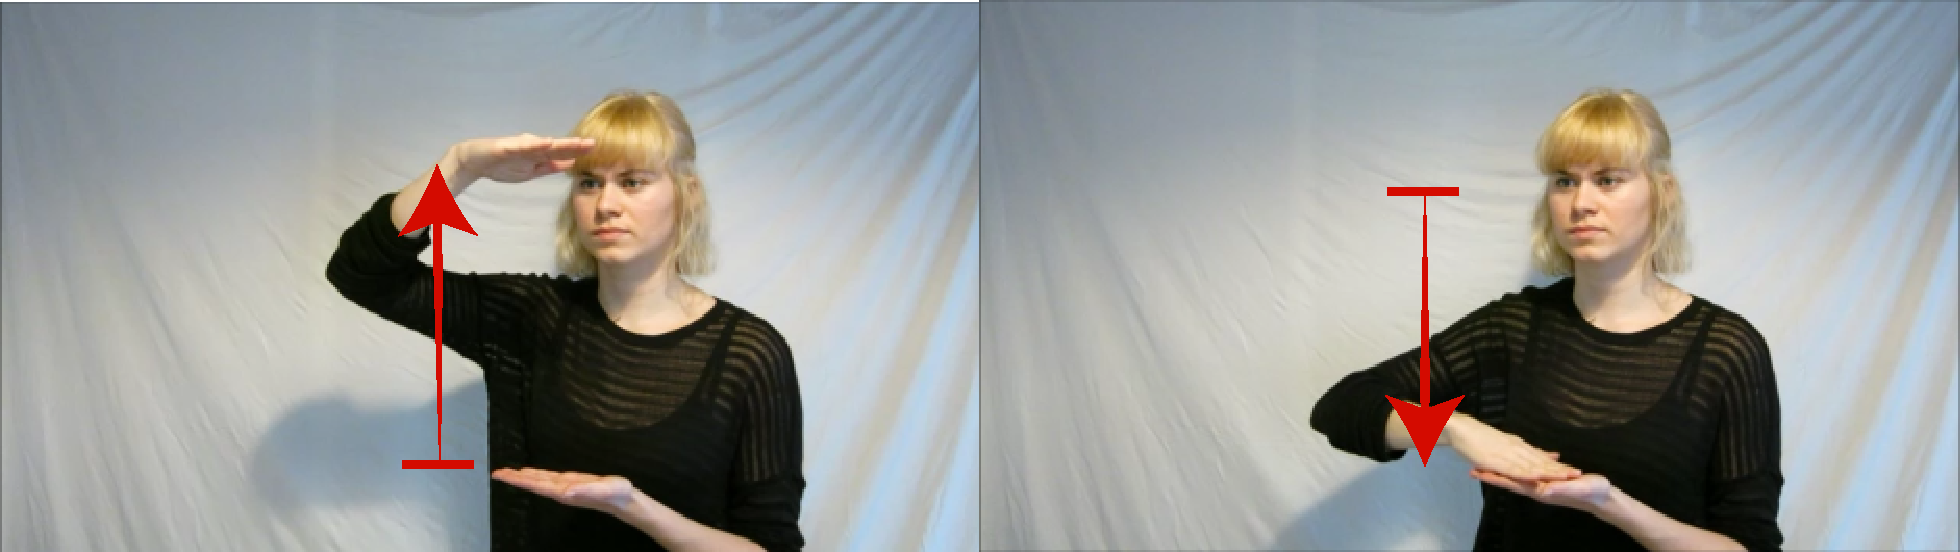
\includegraphics[resolution=300,width=0.9\textwidth]{Test1/Gestik-par/Gestik5_Volumen}
	\caption{Illustration af gestik-par 5; horisontal ikke-dominant hånd med håndfladen opad holdes stationær, mens den dominante hånd ligeledes holde horisontal med håndfladen nedad men løftes vertikalt væk fra den ikke-dominante hånd for at skrue op og sænkes mod den ikke-dominante hånd for at skrue ned.}
	\label{fig:GestikPar5Volumen}
\end{figure}
\noindent
%
Ifølge TP5 og TP7, så tillader GP5 mere kontrol over, hvor meget lydstyrken justeres, fordi gestikken kræver to hænder. Dog påpeger TP5, at testpersonen føler sig mere udsat ved GP5 sammenlignet med GP6, hvor forskellen mellem de to gestik-par er, at GP6 er horisontal modsat GP5, som er vertikal.\blankline
%
Som tidligere nævnt, foretrækker størstedelen af testpersonerne én-hånds gestikker, hvilket er et stærkt argument for, at ekskludere GP5. Derudover indgår GP5 sammenlagt kun seks gange i testpersonernes samlede top tre og aldrig på en førsteplads, jævnfør \autoref{fig:SamletTopTreVolumen}. Ydermere påpeger TP6 et potentielt problem relateret til GP5. Gestikken påbegyndes på den lydstyrke, som musikken allerede spiller ved, svarende til at hænderne er samlet. Når afstanden mellem hænderne øges, skrues der op og når hænderne samles igen er lydstyrken på det oprindelige niveau, hvilket resultere i, at testpersonen er i tvivl om, hvordan der skrues længere ned for lydstyrken. Testpersonen reflekterer over om, hvorvidt den dominante hånd skal være referencen, mens den ikke-dominante hånd angiver hvor meget der skrues ned. Tages alt dette i betragtning vurderes det, at der er belæg for at ekskludere GP5.
%
\subsection{Testpersonernes begrundelse for valg af gestik-par 9}
\label{TestresultaterValgAfGestikkerBegrundelseGP9Volumen}
% 
Med udgangspunkt i \autoref{fig:SamletTopTreVolumen} tildeles GP9 en førsteplads af to testpersoner, en andenplads af én testperson og en tredjeplads af tre testpersoner. GP9 illustreres på \autoref{fig:GestikPar9Volumen}. De testpersoner, som har tildelt GP9 en første-, anden eller tredjeplads, begrunder det ud fra en kombination af følgende egenskaber: 
%
\begin{multicols}{3}
    \begin{itemize}
        \item Smart
        \item Sej
        \item Naturligt
        \item Logisk
        \item Hurtig
        \item Simpel 
        \item Nem
\end{itemize}
\end{multicols}
\noindent
%  
I forhold til de resterende gestik-par er en gennemgående tendens, at GP9 kendetegnes og beskrives som værende både smart og sej.
%
\begin{figure}[H]
	\centering
	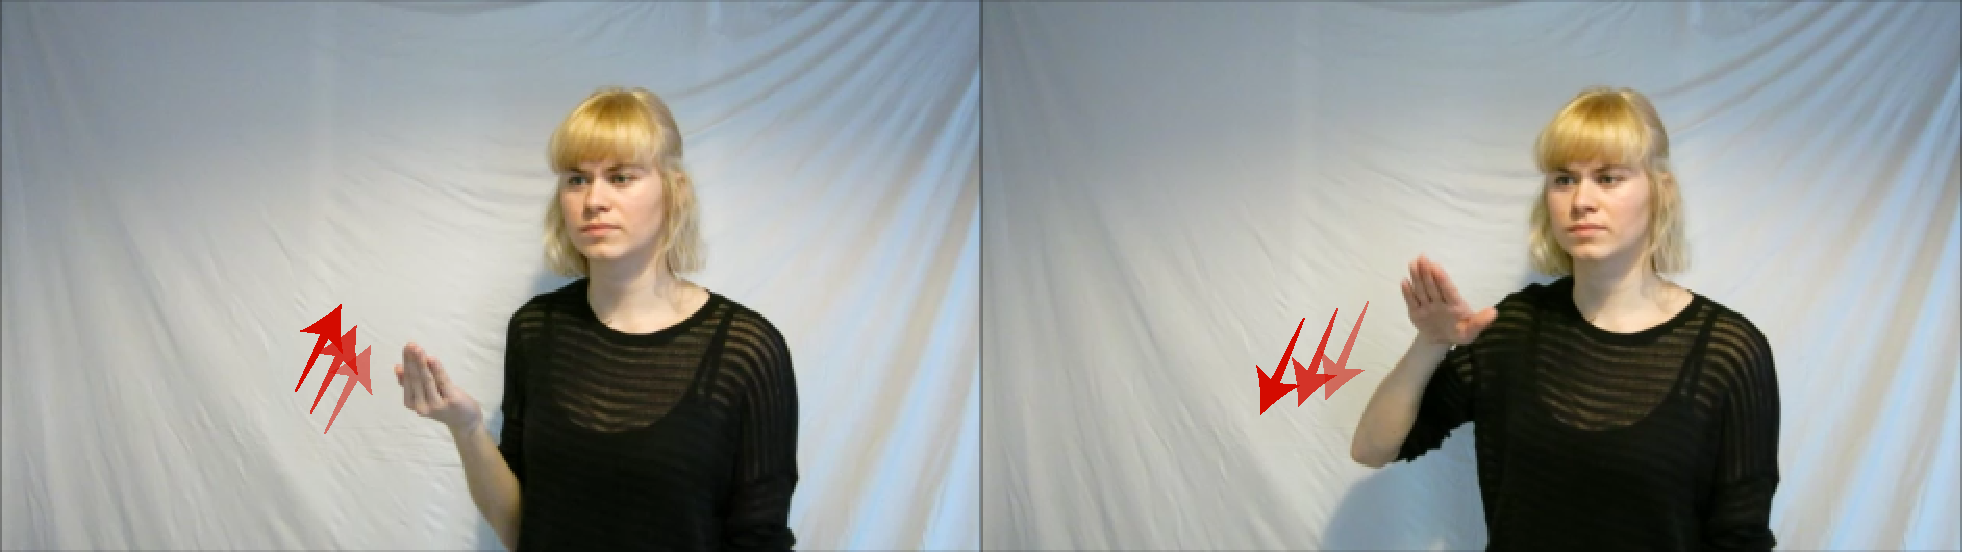
\includegraphics[resolution=300,width=0.9\textwidth]{Test1/Gestik-par/Gestik9_Volumen}
	\caption{Illustration af gestik-par 9; \enquote{kom så}-bevægelse med fingrene for at skrue op og \enquote{ro på}-bevægelse med fingrene for at skrue ned.}
		\label{fig:GestikPar9Volumen}
\end{figure}
\noindent
%
Derudover har hverken TP3 eller TP9 fremsat forbedringsforslag til GP9, men i begge tilfælde har testpersonerne oprindeligt valgt et andet gestik-par ind til de gengiver bevægelserne og begge konkluderer, at GP9 skal tildeles førstepladsen.\blankline
%    
Med udgangspunkt i testpersonernes argumenation for, hvorfor de har valgt GP9 og taget i betragtning af, at GP9 sammenlagt indgår seks gange i testpersonernes samlede top tre, jævnfør \autoref{fig:SamletTopTreVolumen}, samt at gestik-parret er fravalgt to gange, jævnfør \autoref{app:TestresultaterVolumenDaarlig}, vurderes det, at der er belæg for at ekskludere GP9. Ydermere påpeger TP7, at ved GP9 er der ingen kontrol over justeringen af lydstyrken, da det potentielt kan være hvilken som helst lydstyrke testpersonen ender på ved GP9. 
%
\subsection{Valg af gestik-par til at justere lydstyrken}
\label{TestresultaterValgAfGestikkerValgVolumen}
%
Baseret på foregående analyse af hvilket semaforisk gestik-par, der skal knyttes til at justere lydstyrken, er det ikke muligt, endegyldigt at udpege et enkelt gestik-par. Valget står mellem GP2, GP3 og GP4, illustreret på henholdvis \autoref{fig:GestikPar2Volumen}, \autoref{fig:GestikPar3Volumen} og \autoref{fig:GestikPar4Volumen}. Fordelen ved at vælge GP2 er, at det ikke er en bevægelse, som normalvist indgår i ens kropsprog, hvorfor det forventes at risikoen for, at bevægelsen gengives ved en fejl er mindre end ved både GP3 og GP4. En anden fordel ved at vælge GP2 er, at størstedelen af testpersonerne forbinder gestikken med den fysiske interaktion med drejeknappen på et musikanlæg. I denne sammenhæng vælges det derfor, at knytte GP2 til at justere lydstyrken, dog med forbehold for, at GP2 fremover vil gengives mere afslappet sammenlignet med, hvordan GP2 præsenteres i videooptagelsen.    

